\documentclass[pdf, unicode, 12pt, a4paper,oneside,fleqn]{article}
\usepackage[utf8]{inputenc}
\usepackage[T2B]{fontenc}
\usepackage[english,russian]{babel}
\frenchspacing
\usepackage{amsmath}
\usepackage{amssymb}
\usepackage{hyperref}
\usepackage{longtable}
\usepackage[table]{xcolor}
\usepackage{array}
\usepackage{color}
\usepackage{xcolor}
\usepackage{hyperref}
\usepackage{graphicx}
\usepackage{listings}
\lstset{tabsize=2,
    breaklines,
    columns=fullflexible,
    flexiblecolumns,
    numbers=left,
    numberstyle={\footnotesize},
    extendedchars,
    inputencoding=utf8}
\usepackage{longtable}
\def\@xobeysp{ }
\def\verbatim@processline{\hspace{1.2cm}\raggedright\the\verbatim@line\par}
\oddsidemargin=-0.4mm
\textwidth=160mm
\topmargin=4.6mm
\textheight=210mm
\parindent=0pt
\parskip=3pt
\definecolor{lightgray}{gray}{0.9}
\renewcommand{\thesubsection}{\arabic{subsection}}
\lstdefinestyle{customc}{
  belowcaptionskip=1\baselineskip,
  breaklines=true,
  frame=L,
  xleftmargin=\parindent,
  language=C,
  showstringspaces=false,
  basicstyle=\footnotesizettfamily,
  keywordstyle=\bfseries\color{green!40!black},
  commentstyle=\itshape\color{gray},
  identifierstyle=\color{black},
  stringstyle=\color{blue},
}
\lstdefinestyle{customasm}{
  belowcaptionskip=1\baselineskip,
  frame=L,
  xleftmargin=\parindent,
  language=[x86masm]Assembler,
  basicstyle=\footnotesize\ttfamily,
  commentstyle=\itshape\color{purple!40!black},
}
\lstset{escapechar=@,style=customc}
\newcommand{\CWPHeader}[1]{\addtocounter{section}{-1}\section{#1}}
\begin{document}
\section*{Статья в формате TeX о многочленаx Цернике.}
\par\textbf{Задача:} Вычислить первые 5 многочленов и построить их грaфики.
\subsection*{Определения:}
Есть чётные и нечётные многочлены Цернике. Чётные многочлены определены как
$$Z^{m}_{n}(\varphi,p)=R^{m}_{n}(p)*\cos \left(m\,\varphi\right)$$
а нечётные как\\
$$Z^{-m}_{n}(\varphi,p)=R^{m}_{n}(p)*\sin \left(m\,\varphi\right)$$
где m и n — неотрицательные целые числа, такие что n >= m, 
    $\varphi$ — азимутальный угол, а ρ — радиальное расстояние, 0 <= p <= 1.
    Многочлены Цернике ограничены в диапазоне от -1 до +1, т.е
    $\left| {\it Zm\_n}\left(p , \varphi\right)\right| \leq 1$. \\
Радиальные многочлены $R_{n}^{m}$ определяются как\\
$$R_{n}^{m}(p)=\sum_{k=0}^{{{n-m}\over{2}}}{{{\left(-1\right)^{k}\,\left(n-k\right)!\,p^{n-2\,k}}\over{k!\,\left({{n-m}\over{2}}-k\right)!\,\left({{n+m}\over{2}}-k\right)!}}}$$
для чётных значений n - m , и тождественно равны нулю для нечётных n - m .\\
\subsection*{Ортогональность:}
Ортогональность если m = 0:\\
$$\int_{x=0}^1 Z^{m}_{n}(p,\varphi)*Z^{m'}_{n'}(p,\varphi) \,dp = {{\pi}\over{n+1}}$$\\
Ортогональность если m $\neq$ 0:\\
$$\int_{x=0}^1 Z^{m}_{n}(p,\varphi)*Z^{m'}_{n'}(p,\varphi) \,dp = {{\pi}\over{2\,n+2}}$$
\subsection*{Примеры:}
Является ортогональным:$$R^{0}_{0}(p) = 1$$
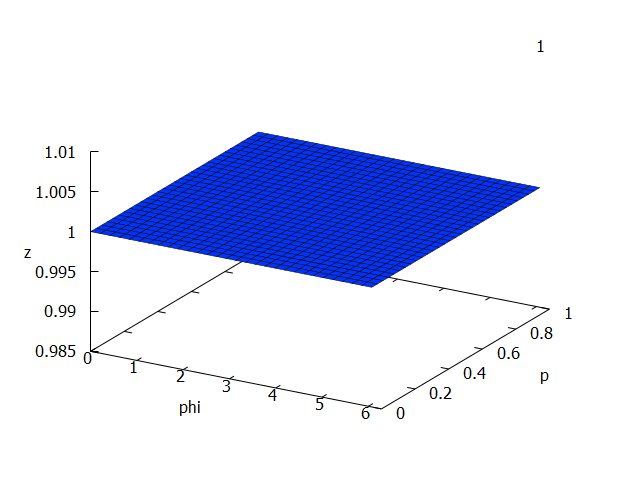
\includegraphics[scale=0.5]{./graph1.png}\\
Не является ортогональным:$$R^{1}_{1}(p) = p\,\cos \varphi$$
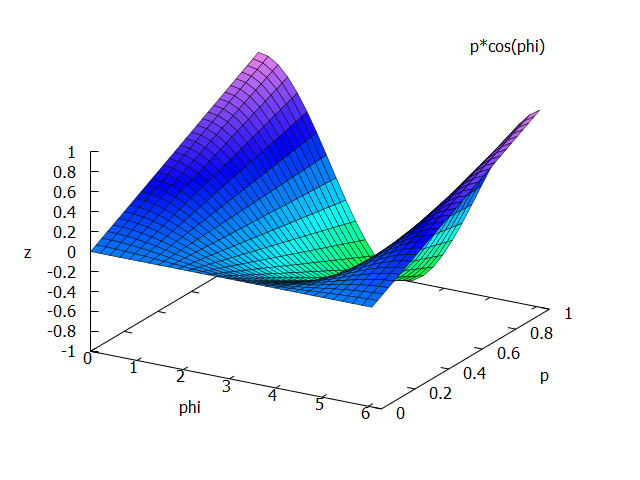
\includegraphics[scale=0.5]{./graph2.png}\\
Является ортогональным:$$R^{0}_{2}(p) = 2\,p^2-1$$
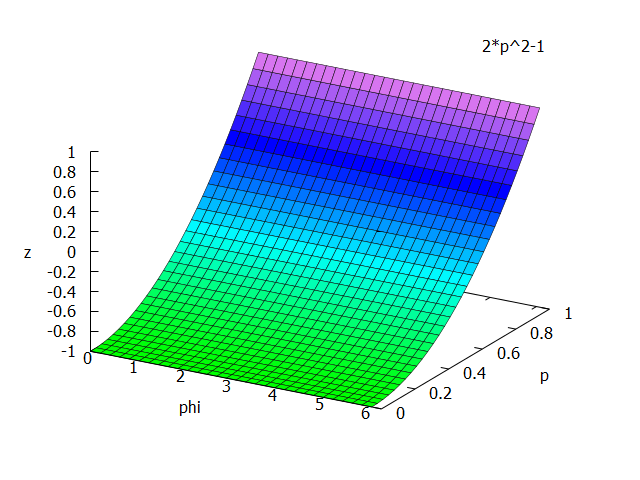
\includegraphics[scale=0.5]{./graph3.png}\\
Не является ортогональным:$$R^{2}_{2}(p) = p^2\,\cos \left(2\,\varphi\right)$$
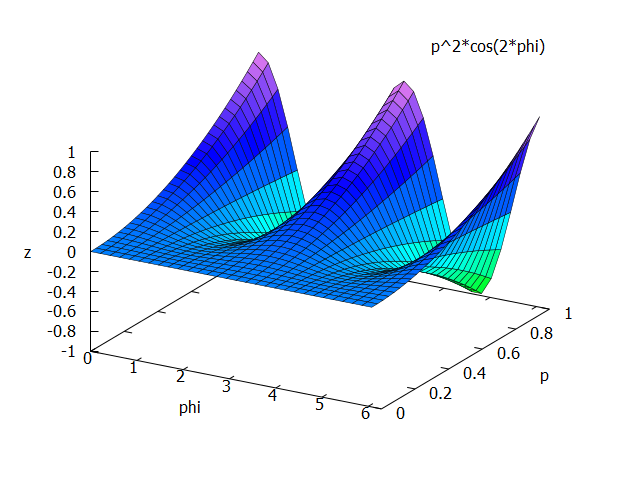
\includegraphics[scale=0.5]{./graph4.png}\\
Не является ортогональным:$$R^{1}_{3}(p) = \left(3\,p^3-2\,p\right)\,\cos \varphi$$
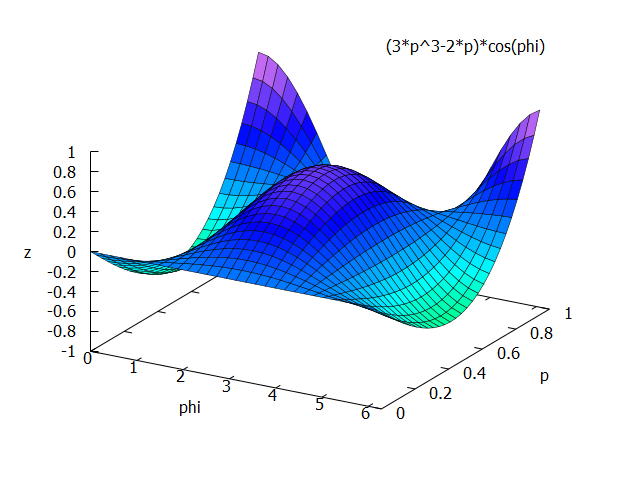
\includegraphics[scale=0.5]{./graph5.png}\\

\end{document}